\documentclass{beamer}
\usepackage[utf8]{inputenc}
\usepackage{graphicx}
\usepackage{hyperref}
\usepackage{amsmath}
\usepackage{amssymb}
\usepackage{amsthm}

\usetheme{Darmstadt}

\title{Basics of astrodynamics}
\subtitle{Tsiolkovsky's rocket equation}
\author{Louis-Hendrik Barboutie}
\institute{University of Luxemburg}
\date{May 2022}

\begin{document}


\begin{frame}
    \maketitle
\end{frame}

\begin{frame}{Table of contents}
    \tableofcontents
\end{frame}

\section{Introduction}
\begin{frame}{Introduction}
    In order to know how far a rocket can go, we need a way to quantify the change in momentum of a rocket.\medskip
    \pause
    
    
    How do we do that?
\end{frame} 

\begin{frame}{Conservation principles}
\begin{block}{Conservation of momentum}
    If no external forces are acting on a system of N bodies, then:
    \begin{equation}
        \frac{d}{dt}\sum_{i=1}^N\Vec{p}_i = 0
    \end{equation}
\end{block}
\pause
\begin{exampleblock}{Newton's second law of motion}
\begin{equation}
    \sum_{i=1}^M \Vec{F}_i = \frac{d}{dt} \Vec{p}_{total}
\end{equation}
\end{exampleblock}
    
\end{frame}

\section{Tsiolkovsky's rocket equation}
\begin{frame}{Tsiolkovsky's equation}
    \begin{definition}
    If a rocket can apply acceleration to itself, the change in momentum $\Delta v$ it undergoes is described by following equation:
        \begin{equation}
            \Delta v = I_{sp} g_0 \ln \left( \frac{m_{\text{initial}}}{m_{final}} \right)
        \end{equation}  
    \end{definition}
    where
    \setbeamercovered{transparent}
        \begin{itemize}
            \item \onslide<2-> $I_{sp}$ is the exhaust specific impulse
            \item \onslide<3-> $g_0$ is the standard gravity
            \item \onslide<4-> $m_{\text{initial}}$ is the mass of the rocket before the burn
            \item \onslide<5-> $m_{\text{final}}$ is the mass of the rocket after the burn
        \end{itemize}
    \setbeamercovered{invisible}
\end{frame} 

\section{Remarks}
\begin{frame}{Remarks}
\begin{columns}
    \column{0.5\textwidth}
    \begin{itemize}
        \item In atmosphere, the specific impulse is variable, thus the $\Delta v$ in vacuum is greater than at sea level, for a same rocket.
        \item For higher $\Delta v$, the ratio of masses has to grow exponentially, ie. double the amount of fuel won't yield double the $\Delta v$.
    \end{itemize}
    \column{0.5\textwidth}
    \begin{figure}
        \centering
        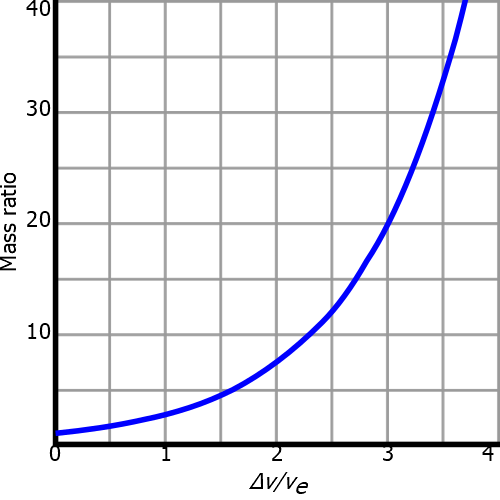
\includegraphics[width=\textwidth]{Tsiolkovsky_rocket_equation.png}
        \caption{mass ratio as function of delta-v}
        \label{fig:equation}
    \end{figure}
\end{columns}
\end{frame}

\section{Examples}
\begin{frame}{Examples}
    \begin{columns}
        \column{0.5\textwidth}
        \begin{figure}
            \centering
            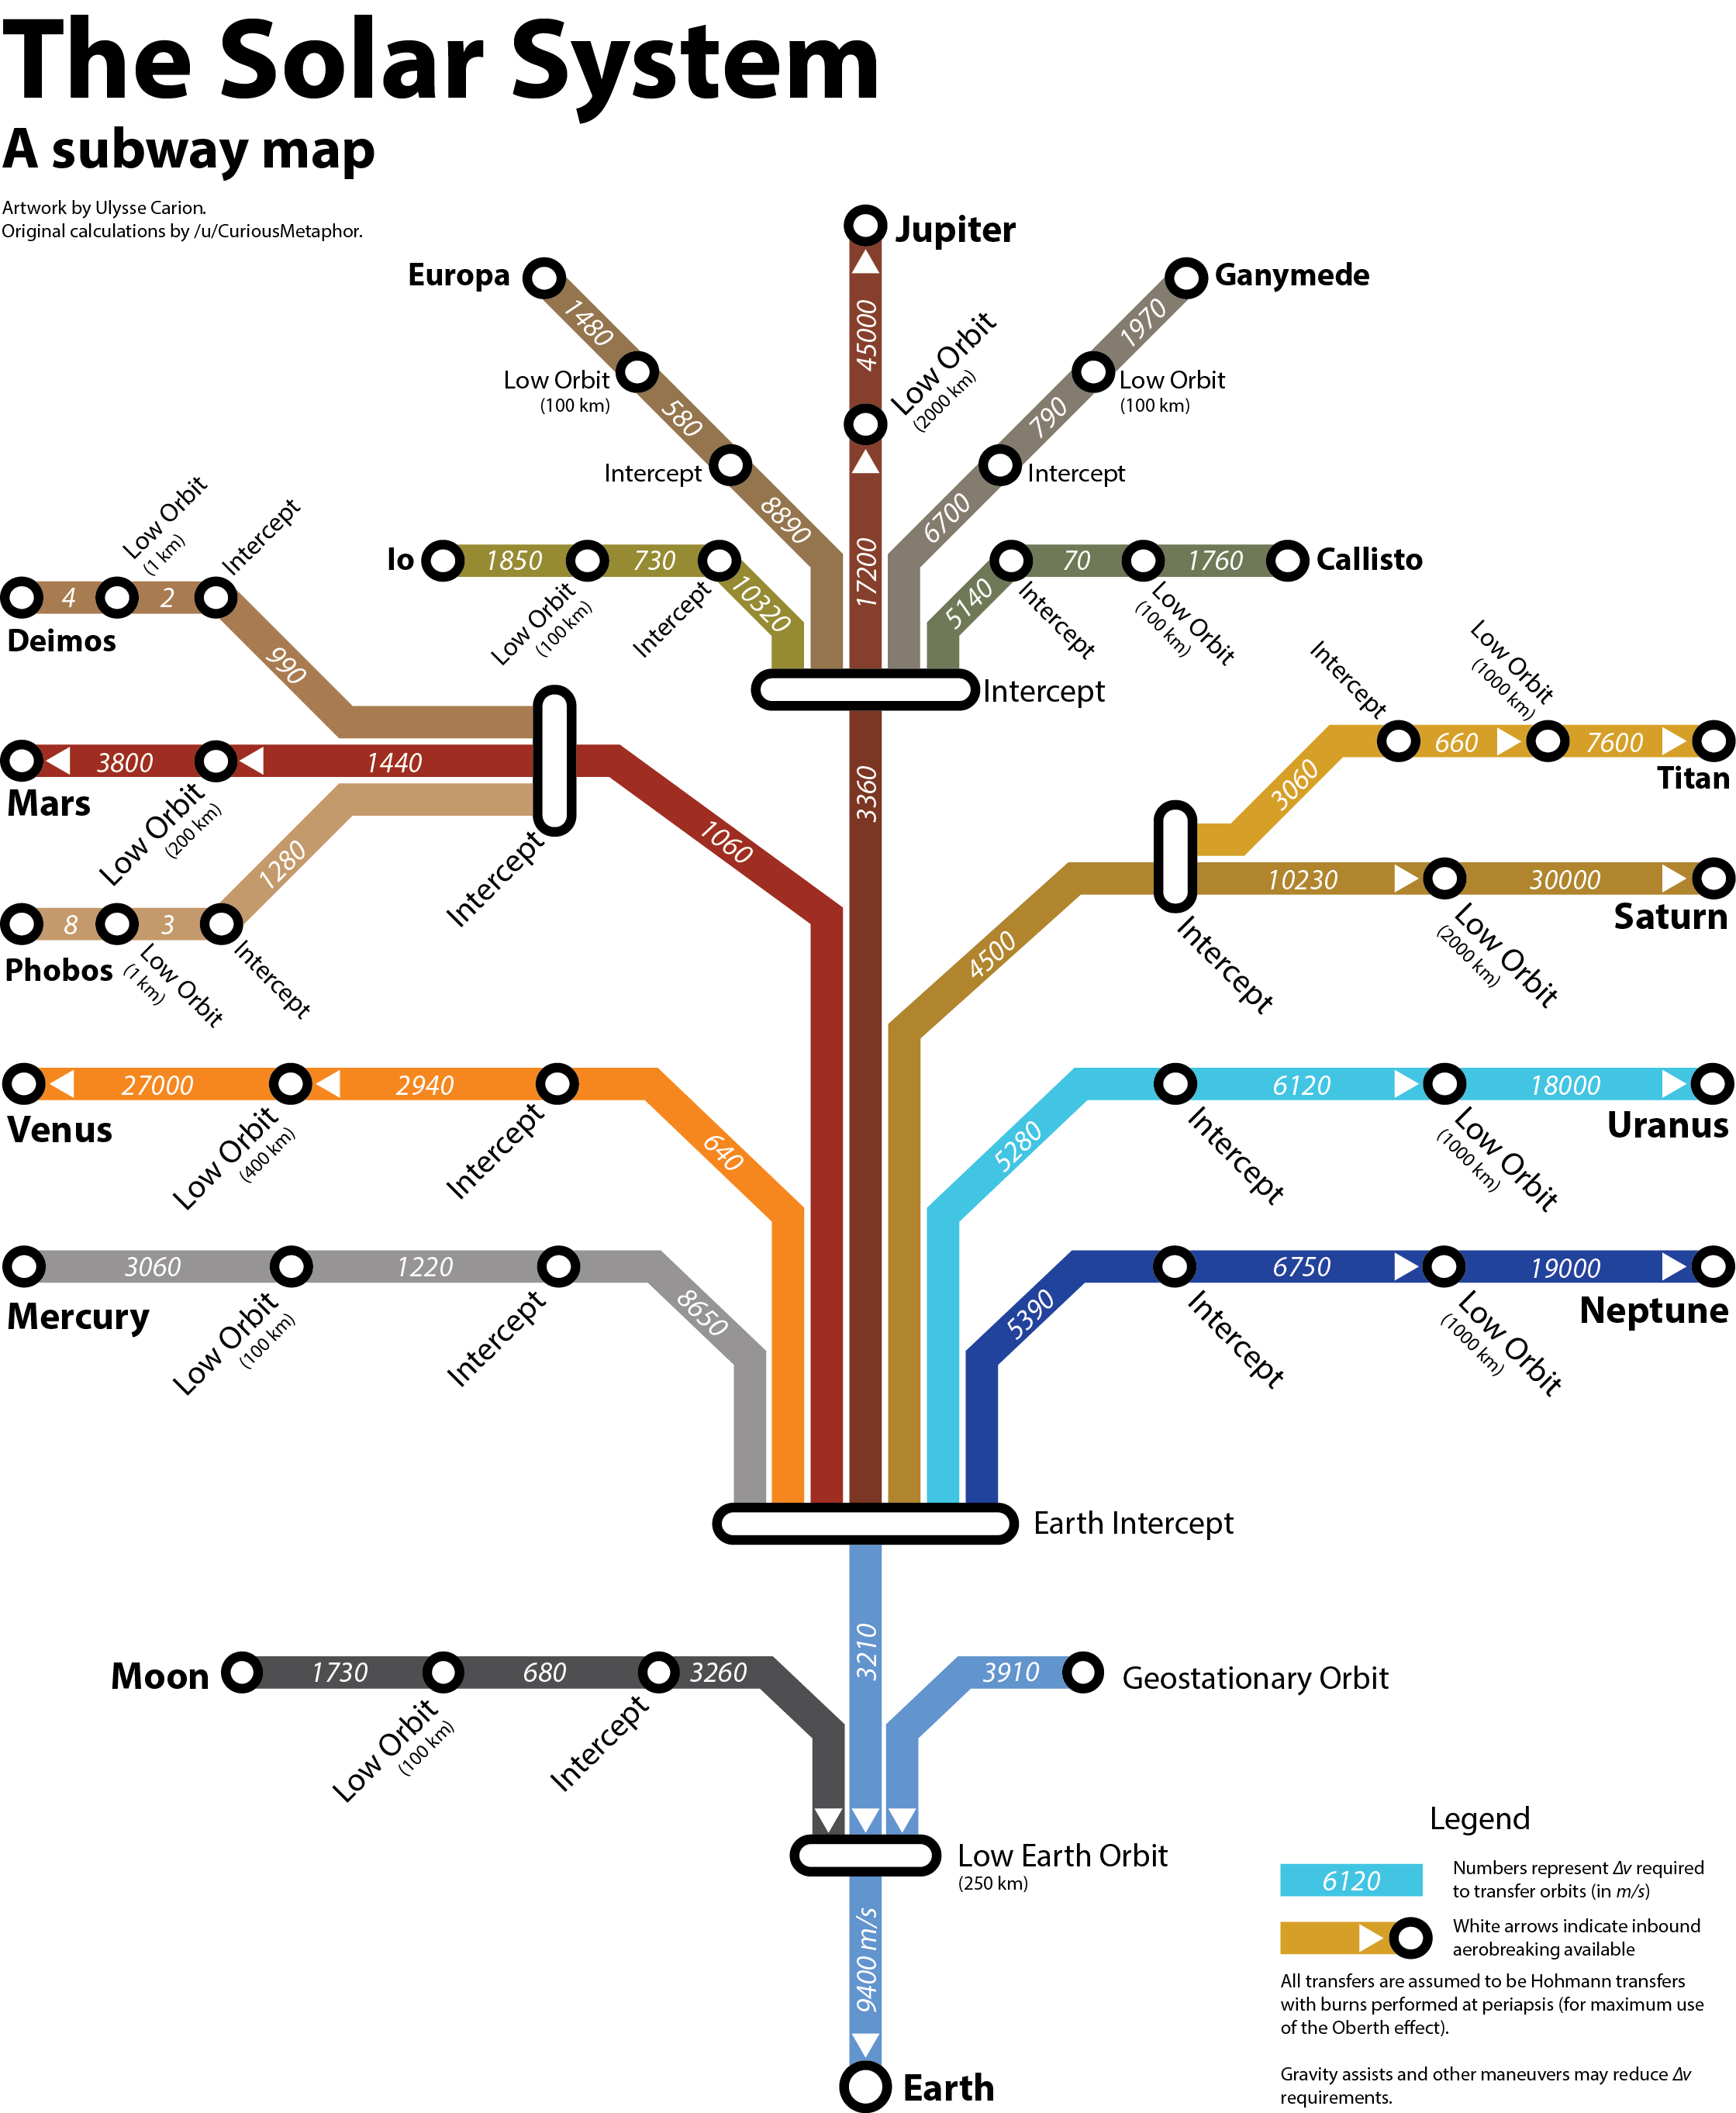
\includegraphics[width=\textwidth]{AAGJvD1.png}
            \caption{$\Delta v$ map of the solar system}
            \label{fig:my_label}
        \end{figure}
        \column{0.5\textwidth}
        Using this map, one can find the required $\Delta v$ to get to other celestial bodies, from flybys to full orbital captures. Getting to low Earth orbit requires 9400~ms$^{-1}$, while a capture around the Moon requires an additional 5670~ms$^{-1}$. Each trip is additive, so to know the total needed $\Delta v$, we add each bit together. 
    \end{columns}   
\end{frame}

\section{References}
\begin{frame}{References}
\begin{thebibliography}{9}
    \bibitem{deltavmap} \url{https://www.reddit.com/r/space/comments/29cxi6/i_made_a_deltav_subway_map_of_the_solar_system/}
    \bibitem{massRatio} \url{https://commons.wikimedia.org/wiki/File:Tsiolkovsky_rocket_equation.svg}
    \bibitem{song} \textit{You will not go to space today}, Skye Manley, \url{https://www.youtube.com/watch?v=Ayu0GsrvKQA}
    \bibitem{knowledge} My own knowledge, \textit{deal with it}.
\end{thebibliography}
\end{frame}

\end{document}